% Dies ist Teil der Vorlesung Physik auf dem Computer, SS 2012,
% Axel Arnold, Universitaet Stuttgart.
% 
% Dieses Werk ist unter einer Creative Commons-Lizenz vom Typ
% Namensnennung-Weitergabe unter gleichen Bedingungen 3.0 Deutschland
% zugänglich. Um eine Kopie dieser Lizenz einzusehen, konsultieren Sie
% http://creativecommons.org/licenses/by-sa/3.0/de/ oder wenden Sie sich
% schriftlich an Creative Commons, 444 Castro Street, Suite 900, Mountain
% View, California, 94041, USA.

\chapter{Optimierung}
\index{Optimierung}

Bei der Optimierung betrachtet man eine Funktion $f:M\to R$, die
\emph{Zielfunktion}, mit einer beliebigen \emph{zulässigen Menge} $M$.
Gesucht ist $x\in M$, so dass $f(x) \le f(x')$ für alle $x'\in M$. Man
schreibt kurz
\begin{equation}
  \label{eq:min}
  \min_{x\in M} f(x).
\end{equation}
Die Menge $M$ ist dabei oft eine Teilmenge des $\RR^n$, die zum
Beispiel durch \emph{Nebenbedingungen} der Form $g(x)\ge 0$
beschrieben wird.

Ein Beispiel einer solchen Aufgabe haben wir bereits im Zusammenhang
mit Funktionsfits kennengelernt. Bei diesem Problem sind Daten $(x_i,
y_i)\in\RR^{m+1}$, $i=1(1)n$ sowie eine parametrisierte Funktion
$f_v(x)$ gegeben, wobei $v$ freie Parameter sind. Gesucht
wird dann
\begin{equation}
  \label{eq:fit}
  \min_{v} \sum_{i=1}^n (f_v(x_i) - y_i)^2.
\end{equation}

Im Spezialfall, dass $f_v$ linear ist, also von der Form
$f_{\tilde{v},v_0}(x) = \tilde{v}^Tx + v_0$, ergibt sich die Aufgabe
\begin{equation}
  \label{eq:min2}
  \min_{(\tilde{v},v_0)\in\RR^{m+1}} \sum_{i=1}^n (\tilde{v}^Tx_i -
  v_0 - y_i)^2 = \min_{v\in\RR^{m+1}} \norm{A v - b}_2.
\end{equation}
mit
\begin{equation*}
  b =
  \begin{pmatrix}
    y_1\\
    \vdots\\
    y_n
  \end{pmatrix}
\quad\text{und}\;
A =
\begin{pmatrix}
  (x_1)_1 & \ldots & (x_1)_m & 1\\
  \vdots &        & \vdots & \vdots\\
  (x_n)_1 & \ldots & (x_n)_m & 1\\
\end{pmatrix}.
\end{equation*}

Die klassische lineare Regression benutzt die 2-Norm und versucht
damit, die mittlere Abweichung zu minimieren. Bei bestimmten Aufgaben
ist aber nicht der mittlere, sondern der maximale Fehler
ausschlaggebend. Dies ist zum Beispiel der Fall bei der
Kraftfeldoptimierung für Molekulardynamiksimulationen, bei der eine
Parametrisierung eines Potentials gesucht wird, die bekannte
experimentelle Daten möglichst gut wiedergibt. Offenbar ist die Güte
einer solchen Näherung durch den maximalen Fehler in einer Eigenschaft
bestimmt und nicht durch den durchschnittlichen Fehler.  Aus
\eqref{eq:min2} wird dann
\begin{equation}
  \label{eq:mininf}
  \min_{v\in\RR^{m+1}} \norm{A v -
    b}_\infty = \min_{v\in\RR^{m+1}} \max_{i=1}^n \abs{(A v)_i - b_i}.
\end{equation}
Obwohl sich scheinbar nicht viel geändert hat, hat dieses Problem
tatsächlich eine ganz andere Struktur, für die andere Lösungsmethoden
benutzt werden. Um dies zu verstehen, fügen wir eine weitere Variable
$v_{m+2}$ zum Parameterraum hinzu. Diese soll nun stets $v_{m+2} =
\norm{A v - b}_\infty$ erfüllen, also $-v_{m+2}\le (A v)_i - b_i \le
v_{m+2}$ für $i=1(1)n$. Damit wird aus \eqref{eq:mininf} eine
Minimierungsaufgabe mit linearer Zielfunktion und Nebenbedingungen:
\begin{equation}
  \label{eq:chebyshevappr}
  \min_v (0,\ldots,\,0,\,1)^T v\quad\text{unter der Bedingung}\;
  \begin{pmatrix}
    A  & e\\
    -A & e
  \end{pmatrix} v \ge
  \begin{pmatrix}
    b\\
    -b
  \end{pmatrix},
\end{equation}
wobei $e=(1,\ldots,1)^T$. Eine solche Aufgabe heißt auch
\emph{\keyword{lineares Programm}} und wird mit Verfahren wie den
Simplexalgorithmus behandelt. Lineare Programme spielen auch in der
Spiele- und Wirtschaftstheorie eine große Rolle.

Die ursprünglich gestellte Aufgabe \eqref{eq:min} oder auch
\eqref{eq:fit} sehen in ihrer allgemeinen Form natürlich auch
nichtlineare Funktionen vor, etwa wenn aufgrund theoretischer
Vorhersagen eine Exponentialfunktion an Daten angeglichen werden soll.
Sofern die Zielfunktion zweifach stetig differenzierbar ist, ist aus
der Analysis ist bekannt, dass im Minimum die Ableitung
verschwindet. Die Nullstellensuche lässt sich im Prinzip mit Hilfe des
Newtonverfahrens behandeln, wir lernen aber noch weitere, auf die
Optimierung zugeschnittene Varianten kennen.

Wie wir gesehen hatten, konvergiert das Newtonverfahren im allgemeinen
nur lokal. Zusätzlich kann eine Nullstelle der Ableitung auch zu einem
Maximum oder Sattelpunkt gehören. Solche Optimierungsverfahren heißen
dann \emph{lokal}\index{Optimierung>lokale} und finden im allgemeinen
nicht das \emph{globale} Minimum \eqref{eq:min}. Dies gilt
insbesondere, wenn Nebenbedingungen gegeben sind, weil sich dann das
Minimum auch irgendwo auf dem Rand der zulässigen Menge befinden
kann. Trotzdem spielen lokale Optimierungsmethoden eine wichtige
Rolle, etwa bei der Energieminimierung. Bei diesem ersten Schritt
typischer Molekulardynamiksimulationen werden die Teilchen zunächst so
verschoben, dass die Energie lokal minimiert wird. Dadurch kann die
eigentliche Simulation mit größeren Zeitschritten begonnen
werden. Eine globale Optimierung ist dabei unnötig, da das System
während der Simulation sowieso nicht im Energieminimum verharrt,
sondern einen hoffentlich ausreichend großen Teil des Phasenraums
besucht.

Die globale Optimierung\index{Optimierung>globale}, also die Suche
nach dem kleinsten lokalen Minimum, ist hingegen vor allem bei der
Suche nach Grundzuständen wichtig. Auch viele praktische Probleme,
etwa die Fahrplanoptimierung, sind globale
Optimierungsprobleme. Leider gibt es hier keine Verfahren mit
gesicherten Konvergenzaussagen, wir werden aber zwei physikalisch
bzw. biologisch motivierte Verfahren kennenlernen.

\section{\keyword{Pseudoinverse}}
\index{Moore-Penrose-Inverse}

Wir betrachten zunächst lineare Optimierungsprobleme der Form
\begin{equation}
  \label{eq:optnorm2}
  \min_{x\in\RR^n} \norm{Ax-b}_2,
\end{equation}
d.h., wir suchen den Vektor $x$, so dass $Ax$ möglichst nahe an $b$
liegt, wobei $A\in\RR^{m,n}$ und $b\in\RR^{m}$.  Solche Probleme
ergeben sich zum Beispiel bei der Ausgleichsrechnung
\eqref{eq:min2}.

Ist $m = n$ und $A$ regulär, so ist die Lösung unmittelbar klar,
nämlich $A^{-1}b$. Ist aber $m>n$, dann ist das Gleichungssystem
$Ax=b$ im allgemeinen nicht lösbar; \eqref{eq:optnorm2} besagt dann,
dass wir dasjenige $x$ suchen, dass das Gleichungssystem möglichst gut
löst.

Ist umgekehrt $m < n$, so ist das Gleichungssystem im allgemeinen
nicht eindeutig zu lösen. Wir können nun aber die Lösung minimaler
Norm $\norm{x}$ suchen. Dies führt zu einer Optimierungsaufgabe mit
Nebenbedingungen:
\begin{equation}
  \label{eq:optnorm2bild}
  \min_{x\in\RR^n} \norm{x}_2\quad\text{unter der Bedingung}\; Ax=b.
\end{equation}

Um Aufgabe \eqref{eq:optnorm2} zu lösen, formen wir sie zunächst etwas um:
\begin{equation}
  \norm{Ax - b}^2_2 = (Ax - b)^T(Ax - b)
  = x^TA^TAx - 2b^TAx + b^Tb.
\end{equation}
Es handelt sich also um eine quadratische Optimierungsaufgabe, deren
Minimum $x$
\begin{equation}
  \nabla \norm{Ax - b}^2_2 = \left(\frac{\partial}{\partial x_i} \norm{Ax -
    b}^2_2\right)_i = 2x^TA^TA - 2b^TA = 0
\end{equation}
erfüllt. Hat $A$ linear unabhängige Spalten, so ist $A^TA$ invertierbar,
und wir finden die Lösung als
\begin{equation}
  x = (A^TA)^{-1}A^Tb.
\end{equation}

Die zweite Aufgabe, \eqref{eq:optnorm2}, können wir ganz ähnlich
lösen. In diesem Fall hat $A$ weniger Zeilen als Spalten, ist also
unterbestimmt. Hat $A$ aber wengistens linear unabhängige Zeilen, so
ist $AA^T$ invertierbar, und wir können
\begin{equation}
  x = A^T(AA^T)^{-1}b
\end{equation}
definieren. Dann erfüllt $x$ offenbar die Nebenbedingung $Ax=b$, und
alle anderen zulässigen $x'$ liegen in $x + \text{Kern}(A) = x +
\text{Bild}(A^T)^\perp$. Da $x\in\text{Bild}(A)$, gilt
$\norm{x'}=\norm{x} + \norm{x-x'}\ge \norm{x}$. Mit anderen Worten,
$x$ löst die Optimierungsaufgabe \eqref{eq:optnorm2bild}.

Die Matrizen $(A^TA)^{-1}A^T$ und $A^T(AA^T)^{-1}$ sind Spezialfälle
der \emph{Pseudoinversen} oder \emph{Moore-Penrose-Inversen} für
allgemeine Matrizen. Der Name Pseudoinverse rührt daher, dass diese
unter den gegebenen Nebenbedingungen die Gleichungen, so gut es geht,
invertieren, die Pseudoinverse findet also das $x$ mit minimaler Norm
unter allen $x$, für die $\norm{Ax-b}_2$ minimal ist.  Moore und
Penrose haben abstrakte Bedingungen für die Pseudoinverse definiert,
die von den obigen Ausdrücken erfüllt werden. Die Pseudoinverse für
beliebige Matrizen kann durch eine sogenannte Singulärwertzerlegung
bestimmt werden kann. Diese kann in dieser Vorlesung leider nicht
behandelt werden, aber wir werden jetzt sehen, wie man bei Matrizen
mit maximalem Zeilen- oder Spaltenrang die Pseudoinverse auch mit
Hilfe der QR-Zerlegung bestimmt werden kann, ohne $A^TA$ oder $AA^T$
berechnen und invertieren zu müssen.

Sei also $A\in\RR^{m,n}$ eine Matrix mit maximalem Spaltenrang,
insbesondere $m \ge n$. Aus dem Householder- oder Givensverfahren
erhalten wir
\begin{equation}
  A = 
  \begin{pmatrix}
    Q_1 & Q_2
  \end{pmatrix}
  \cdot
  \begin{pmatrix}
    R_1\\
    0
  \end{pmatrix},
\end{equation}
wobei $R_1$ eine reguläre rechte obere $n\times n$-Dreiecksmatrix ist,
und $Q_1$ die zugehörigen $n$ ersten Spalten der unitären Matrix $Q$.
Dann ist
\begin{equation}
  (A^TA)^{-1}A^Tb = (R_1^TQ_1^TQ_1 R_1)^{-1}A^Tb =
  R_1^{-1}\left(R_1^T\right)^{-1}A^Tb,
\end{equation}
was durch bequemes Vorwärts- und Rückwärtseinsetzen ohne
Matrixinversion gelöst werden kann. Wie man sieht, ist in diesem Fall
die genaue Form der Matrix $Q$ unerheblich.

Hat umgekehrt $A$ maximalen Zeilenrang, insbesondere also $m \le n$,
dann zerlegen wir $A^T$ mit Hilfe von Householder- oder
Givensverfahren wie oben in eine reguläre rechte obere $m\times
m$-Dreiecksmatrix $R_1$ und orthonormale Matrizen $Q_1\in\RR^{n,m}$
und $Q_2\in\RR^{n,n-m}$. Dann gilt entsprechend
\begin{equation}
  A^T(AA^T)^{-1}b = A^T(R_1^TQ_1^TQ_1 R_1)^{-1}b =
  A^TR_1^{-1}\left(R_1^T\right)^{-1}b.
\end{equation}

Für Zielfunktionen von der Form $\norm{Ax-b}_2$, also gewissermaßen
das Optimierungs-Äquivalent von linearen Gleichungssystemen, lässt
sich also das Optimierungsproblem mit Hilfe der QR-Zerlegung lösen.

\section{Nichtlineare Optimierung}

Für nichtlineare, aber wenigstens zweifach stetig differenzierbare
Zielfunktionen $f:\RR^n\to \RR$ gilt in freien Minima $x$
\begin{equation}
  \nabla f(x) = 0.
\end{equation}
Für diese Gleichung können wir das mehrdimensionale Newtonverfahren
formulieren. Wir wählen also einen Startpunkt $x^{(0)}$ in der Nähe
des Minimums und setzen
\begin{equation}
  x^{(k+1)} = x^{(k)} - f''\left(x^{(k)}\right)^{-1}\nabla f\left(x^{(k)}\right),
\end{equation}
wobei
\begin{equation}
  f''(x) = 
  \left(\frac{\partial^2}{\partial x_j\partial x_k}f(x)\right)_{k,j} = 
  \begin{pmatrix}
    \frac{\partial^2}{\partial x_1^2}f(x) & \ldots &
    \frac{\partial}{\partial x_1\partial x_n}f(x)\\
    \vdots               &        & \vdots \\
    \frac{\partial}{\partial x_1\partial x_n}f(x) & \ldots &
    \frac{\partial^2}{\partial x_1^2}f(x)
  \end{pmatrix}.
\end{equation}
Bei großen Dimensionen $n$ kann es rasch sehr aufwendig werden,
$f''(x)$ zu berechnen, dies ist aber auch nötig, um zu überprüfen,
ob das gefundenene Extremum auch tatsächlich ein Minimum ist. Daher
ist dieses Verfahren nicht optimal. Besser sind die folgenden
Verfahren, die ohne $f''(x)$ auskommen.

\subsection{\keyword{Verfahren des steilsten Abstiegs}}
\index{Gradientenabstiegsverfahren}

Da das Newtonverfahren, das wir oben auf die Ableitung angewendet
haben, auf einer Taylorentwicklung erster Ordnung
basiert, basiert die Optimierung mit Hilfe des Taylorverfahrens in
gewisser Weise auf einer Taylorentwicklung zweiter Ordnung. Was können
wir nun mit der praktikableren Taylorentwicklung erster Ordnung
erreichen? Diese ist zunächst einmal
\begin{equation}
  \label{eq:steepestdescentexpand}
  f(x + \lambda d) = f(x) + \lambda \nabla f(x)d + \O(\lambda^2)
\end{equation}
für eine Richtung $d$ und \emph{Schrittweite} $\lambda > 0$.  Anders
als beim Newtonverfahren können wir nun nicht das Minimum dieser
Näherung als neue Iterierte benutzen, da die Näherung linear ist und
daher kein Minimum hat. Daher können wir lediglich versuchen, $f$ zu
verringern. Da $\lambda>0$ ist und wir für kleine $\lambda$ die
quadratischen Anteile vernachlässigen können, muss $\nabla f(x)d < 0$
gelten. Eine Richtung $d$, die dies erfüllt, heißt
\emph{Abstiegsrichtung}.

Den maximalen Abstieg erreichen wir,wenn $d = -\nabla f(x)$; diese
Richtung heißt daher auch steilster Abstieg. Für das \emph{Verfahren
  des steilsten Abstiegs} (auch \emph{Gradientenabstiegsverfahren}
wählt man zunächst einen Startwert $x^{(0)}$ und setzt dann
\begin{equation}
  \label{eq:steepestdescent}
  x^{(k+1)} = x^{(k)} - \lambda \nabla f\left(x^{(k)}\right)
\end{equation}
mit einer geeigneten Schrittweite $\lambda>0$. Im einfachsten Falle
ist $\lambda$ einfach eine kleine Konstante, zum Beispiel 0.01.

\subsection{\keyword{Schrittweitensteuerung}}
\index{Armijo-Schrittweite}

Besser ist aber, die Schrittweite so zu wählen, dass das Verfahren
sicher absteigt. Dafür gibt es verschiedene Verfahren, von denen hier
nur die recht effizienten \emph{Armijo-Schrittweiten} besprochen
werden.

Entlang der festgelegten Richtung $d$ ist die Optimierung nur noch ein
eindimensionales Problem, und wegen \eqref{eq:steepestdescentexpand}
gilt in einer kleinen Umgebung von $x$ für alle
$\alpha<\nicefrac{1}{2}$ stets
\begin{equation}
  \label{eq:armijo}
  f(x + \lambda d) \le f(x) + \alpha\lambda \nabla f(x)^Td.
\end{equation}
Wir wählen $\lambda$ so, dass diese Bedingung erfüllt ist, und
natürlich möglichst groß. $\alpha\in(0,\,\nicefrac{1}{2})$ bestimmt
dabei den Mindestabstieg, den wir erreichen wollen. Um $\lambda$ zu
bestimmen, beginnen wir einfach mit $\lambda_0=1$, und setzen
anschließend $\lambda_{k+1} = \rho\lambda_{k}$, solange
\eqref{eq:armijo} nicht erfüllt ist. $\rho\in (0,1)$ ist dabei eine
weiter Verfahrenskonstante, die bestimmt, wie rasch wir $\lambda$
verkleinern. Um die Bedingung zu überprüfen, benötigen wir lediglich
die beiden reellen Konstanten $\nabla f(x)^Td$ und $f(x)$ und müssen
in jedem Schritt $f(x + \lambda d)$ neu auswerten.  $\alpha$ wird
meist eher klein gewählt, etwa $0,1$, denn je strikter diese
Bedingung, desto kleiner wird die Schrittweite. Umgekehrt sollte man
$\rho$ nicht zu klein wählen, weil sonst rasch sehr kleine
Schrittweiten benutzt werden.

Die Schrittweitensteuerung setzt nur eine Abstiegsrichtung $d$ voraus,
und kann daher zum Beispiel auch auf das Newton-Verfahren angewandt
werden, dessen Richtung $d=-f''\left(x^{(k)}\right)^{-1}\nabla
f\left(x^{(k)}\right)$ ist. Diese Richtung ist dann eine
Abstiegsrichtung, wenn $\nabla f\left(x^{(k)}\right)
f''\left(x^{(k)}\right)^{-1} \nabla f\left(x^{(k)}\right)$, also, wenn
$f''\left(x^{(k)}\right)^{-1}$ positiv definit ist. Dies ist zumindest
in einer Umgebung eines Minimums der Fall.

\subsubsection{Beispiel: Gradientenabstiegsverfahren mit
  Schrittweitensteuerung}
\label{sec:armijosd}

In Python sieht das Verfahren des steilsten Abstiegs mit
Armijo-Schrittweiten so aus:
\lstinputlisting[firstline=10]{armijo.py}%
Die Funktion \lstinline!armijo_steepest_descent! benötigt dabei als
Eingabeparameter Pythonfunktionen \argd{f} und \argd{gradf}, die die
zu minimierende Funktion und ihren Gradienten zurückliefern. Die
Konstanten \argd{alpha} und \argd{rho} entsprechen den Konstanten
$\alpha$ und $\rho$ des Armijo-Verfahrens. Die Vorgaben $\alpha=0,1$
und $\rho=0,5$ sind übliche Werte, die meist zu guter Konvergenz
führen. Das Verfahren bricht regulär ab, wenn $\norm{\nabla
  f(x^{(k)})}<$ \argd{tol}. Um ein Einfrieren durch zu kleine
Schrittweiten zu vermeiden, wird außerdem eine Mindestschrittweite von
\argd{tol}$^2$ verlangt. Führt diese zu keinem Abstieg mehr, wird
ebenfalls abgebrochen.

\begin{figure}
  \centering
  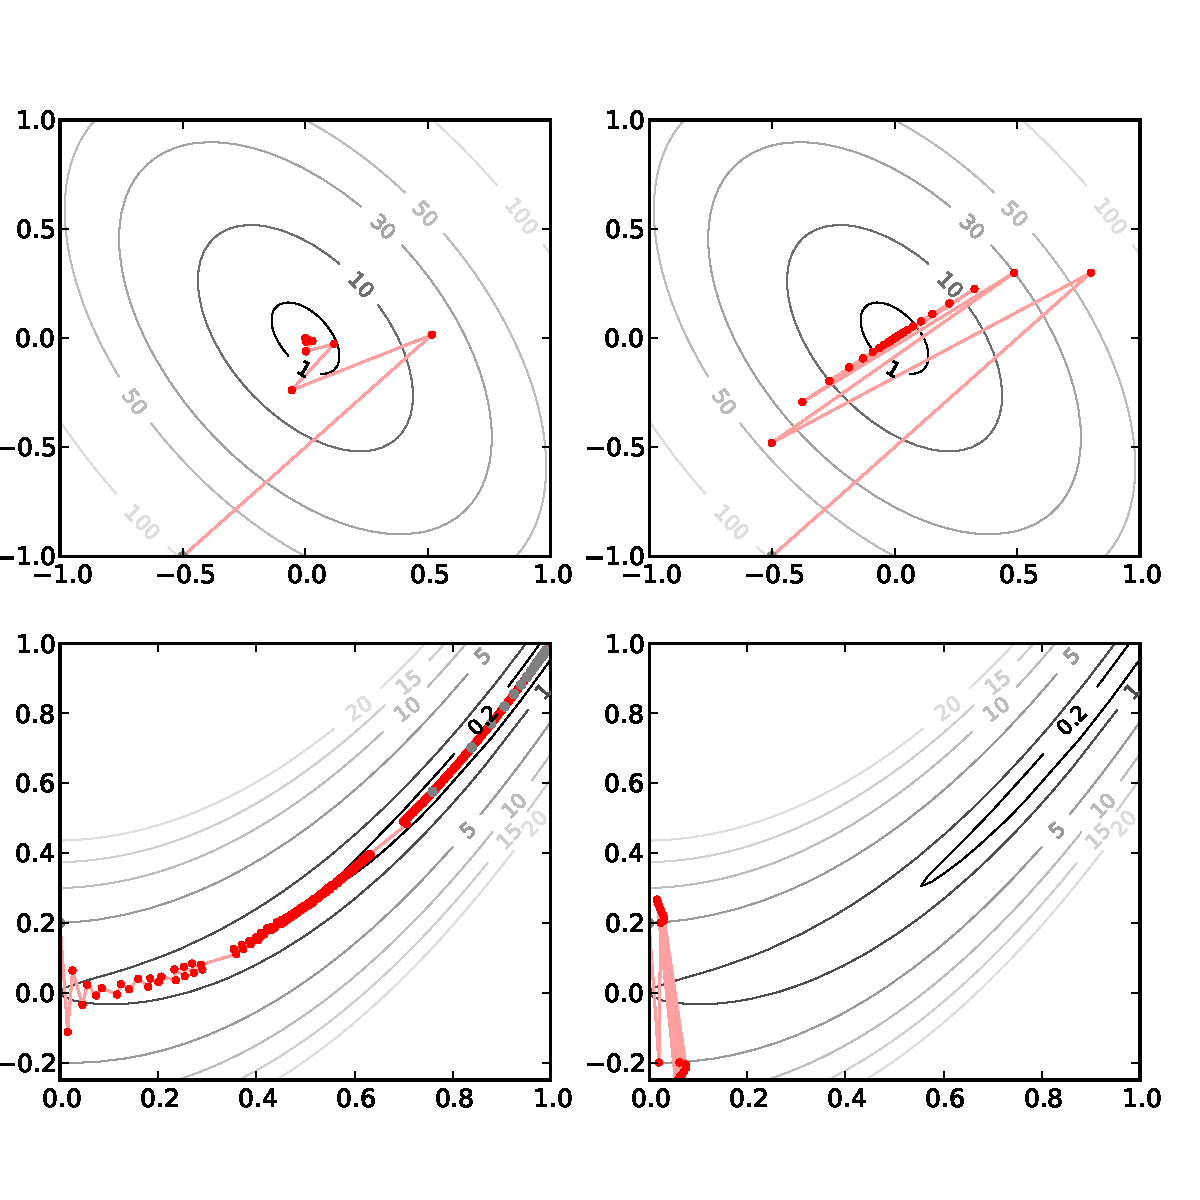
\includegraphics[width=\textwidth]{plots/steepestdescent}
  \caption{Verfahren des steilsten Abstiegs für eine quadratische
    Funktion (oben) und die Rosenbrockfunktion (unten). Links werden
    Armijo-Schrittweiten mit $\alpha=0,1$ und $\rho=0,5$, rechts eine
    konstante Schrittweite von $0,01$ verwendet. Die roten,
    verbundenden Punkte markieren die Iterierten $x^{(k)}$, die
    Höhenlinien illustrieren die zu optimierende Funktion. Für die
    quadratische Funktion konvergieren beide Verfahren gegen das
    Minimum bei $(0,\,0)$, und auch das Armijo-Verfahren wählt eine
    konstante Schrittweite von etwa $0,0078$. Dies hat zur Folge, dass
    das Verfahren wesentlich weniger über das Minimum hinauszielt und
    nur 11 statt 35 Schritte benötigt. Für die Rosenbrockfunktion
    benötigt alleine das schrittweitengesteuerte Verfahren etwa 1700
    Iterationen, um in die Nähe des Minimums bei $(1,1)$ zu kommen.  Jeder
    200. Punkt ist im Graphen grau gefärbt, um die extrem langsame
    Konvergenz zu visualieren. Für die konstante Schrittweite $0,01$
    konvergiert das Verfahren gar nicht, wie die
    eingezeichneten ersten zehn Punkte zeigen.} \label{fig:armijo}
\end{figure}

\index{Rosenbrock-Funktion}%
Als Beispiel betrachten wir das Verfahren des steilsten Abstiegs für
zwei auf der Ebene definierte Funktionen. Die erste Funktion ist eine
quadratische Funktion
\begin{equation}
  \label{eq:quadgl}
  f(x, y) = 40 x^2 + 30(x + y)^2 + 20 y^2,
\end{equation}
die ihr Minimum bei $(0,0)$ hat, die zweite Funktion ist die
Rosenbrockfunktion
\begin{equation}
  f_{\text{Rosenbrock}}(x, y) = (1-x)^2 + 100(y-x^2)^2.
\end{equation}
Diese hat ihr Minimum offenbar bei $(1,1)$, ist aber das
Optimierungsäquivalent zur Rungefunktion. Denn während das Minimum in
einem sehr steilen Tal liegt, ist der Gradient entlang der Talsohle
sehr flach. Die meist gierigen Optimierungsverfahren finden daher sehr
schnell in die Talsohle, kommen dort aber nur noch langsam ins Ziel,
da die Hauptabstiegsrichtung vorwiegend in die Talsohle statt
entlang dieser zeigt.

Abbildung~\ref{fig:armijo} zeigt die Anwendung des Verfahrens des
steilsten Abstiegs mit und ohne Schrittweitensteuerung auf die beiden
Funktionen und illustriert dabei die beiden Hauptschwächen des
Gradientenabstiegsverfahrens. Einerseits neigt es dazu, über das
Minimum hinauszuschießen, und sich dadurch langsam in das Minimum
einzupendeln. Dies lässt sich durch die Schrittweitensteuerung
begrenzen. Andererseits muss der steilste Abstieg nicht in Richtung
des Minimums zeigen, in diesem Fall neigt das Verfahren des steilsten
Abstiegs dazu, sich dem Minimum in Zick-Zack-Kurven mit sehr geringer
Schrittweite zu nähern.

Bei zu großer Schrittweite kann das Verfahren sogar gar nicht
konvergieren. Da von vorneherein die maximale Ableitung meist nicht
bekannt ist, ist also eine Schrittweitensteuerung unerlässlich.

\subsection{\keyword{CG-Verfahren}}
\index{konjugierter Gradient}

Wir betrachten nun einen wichtigen Spezialfall, nämlich quadratische
Funktionen der Form
\begin{equation}
  \label{eq:cgfunktion}
  f(x) = \frac{1}{2}x^TAx - x^Tb
\end{equation}
mit positiv definiter Matrix $A\in\RR^{n,n}$.  Dies bedeutet, dass $A$
symmetrisch ist und $x^TAx>0$ für alle Vektoren $x\neq 0$ erfüllt,
etwa, weil alle Eigenwerte positiv sind.  Positiv definite Matrizen
treten zum Beispiel bei quantenmechanischen Rechnungen auf.

Für Funktionen der Form \eqref{eq:cgfunktion} gibt es ein iteratives
Verfahren, dass bei unbegrenzter Genauigkeit in spätestens $n$
Schritten gegen die exakte Lösung konvergiert. Dieses Verfahren ist
das konjugierte Gradienten-Verfahren (englisch conjugate gradient,
daher kurz auch CG-Verfahren).
Das Optimierungsproblem $\min f(x)$ kann dabei auch als Gleichung
aufgefasst werden, da
\begin{equation}
  Ax = b \quad\iff\quad x\;\text{minimiert}\;f(x) = \frac{1}{2}x^TAx - x^Tb.
\end{equation}
Daher wird das CG-Verfahren auch als effizienter
Gleichungslöser für positiv definite Matrizen behandelt.

Um das Minimum iterativ zu suchen, starten wir mit einem beliebigen
Startwert $x^{(0)}$ (zum Beispiel 0), und verfeinern die aktuelle
Näherung gemäß $x^{(k+1)} = x^{(k)} + \lambda^{(k)}d^{(k)}$ so, dass
wir uns dem Minimum nähern. Wie wir gesehen haben, ist der steilste
Abstieg, also in Richtung des negierten Gradienten $r^{(k)} =
b-Ax^{(k)}$, nicht ideal. Die Idee des CG-Verfahrens ist nun, die
Richtungen $d^{(k)}$ in gewisser Weise stets senkrecht zu einander zu
wählen, so dass Hin- und Herpendeln oder Zick-Zack-Kurse
ausgeschlossen sind. Tatsächlich wählt man die Abstiegsrichtungen
senkrecht in dem durch $A$ induzierten Skalarprodukt, also so, dass
$(d^{(i)}, d^{(k)})_A := \left(d^{(i)}\right)^TAd^{(k)}=0$ für $i\neq
k$. Man sagt auch, dass $d^{(i)}$ und $d^{(k)}$ $A$-konjugiert sind,
daher der Name des Verfahrens.

\begin{figure}
  \centering
  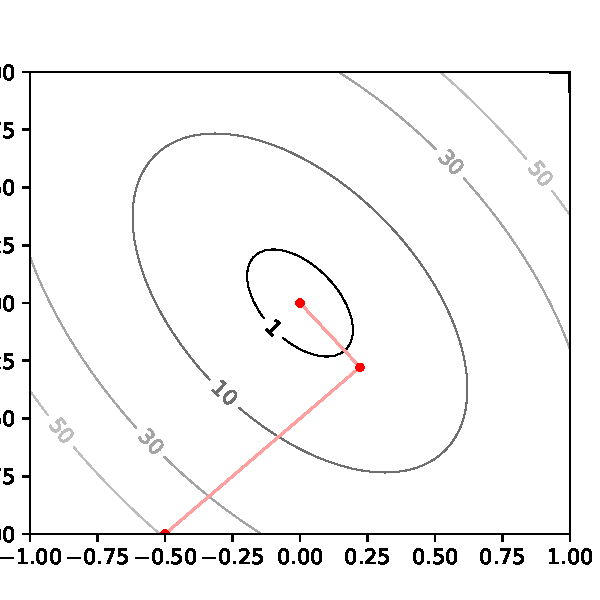
\includegraphics[width=0.5\textwidth]{plots/cg}
  \caption{CG-Verfahren für die quadratische Funktion aus
    \eqref{eq:quadgl}. Die Höhenlinien stellen die zu optimierende
    quadratische Funktion dar, die roten Punkte markieren die
    Iterierten des CG-Verfahrens, das in nur 2 Schritten konvergiert.}
  \label{fig:cg}
\end{figure}

Um dies zu erzwingen, benutzt man das Gram-Schmidt-Verfahren, um die
Gradientenabstiegsrichtungen $r^{(k)}$ zueinander senkrecht bezüglich
$(\cdot,\cdot)_A$ zu machen. Dabei muss aufgrund der Wahl der
Richtungen $d^{(k+1)}$ nur senkrecht zu $d^{(k)}$ gemacht werden, zu
den anderen bisherigen Richtungen steht $d^{(k+1)}$ dann automatisch
senkrecht. Der Vorfaktor kann dabei vereinfacht werden:
\begin{equation}
  \frac{(r^{(k+1)}, d^{(k)})_A}{(d^{(k)}, d^{(k)})_A}
  = -\frac{\left(r^{(k+1)}\right)^Tr^{(k+1)}}{\left(r^{(k)}\right)^Tr^{(k)}}.
\end{equation}

Die Schrittweite kann bei einer quadratischen Funktion so bestimmt
werden, das $\lambda$ die Funktion entlang der Richtung $d$, also
\begin{equation}
  \frac{1}{2}(x+\lambda d)^TA(x+\lambda d) - b^T(x+\lambda d)
  =  \frac{1}{2}x^TAx - b^Tx + \lambda d^T(Ax - b) + \frac{1}{2}\lambda^2 d^TAd,
\end{equation}
minimiert. Es ergibt sich
\begin{equation}
  \lambda^{(k)}  =  \frac{\left(d^{(k)}\right)^Tr^{(k)}}{\left(d^{(k)}\right)^TAd^{(k)}}.
\end{equation}

Zusammengefasst ergibt sich das CG-Verfahren in Python als
\lstinputlisting[firstline=10]{cg.py}%
Das Verfahren bricht ab, wenn $\norm{r^{(k)}} <$ \argd{tol}, anstatt
stur $n$ Schritte zu berechnen, da durch numerische Ungenauigkeiten
unter Umständen 1-2 zusätzlich Schritte nötig werden können. Umgekehrt
können natürlich auch weniger Schritte notwendig sein, wenn der
Startwert günstig liegt.

Abbildung~\ref{fig:cg} illustriert das CG-Verfahren an der selben
quadratischen Funktion, für die das schrittweitengesteuerte
Gradientenabstiegsverfahren 11 Schritte brauchte, um 10 Stellen
Genauigkeit zu erreichen. Das CG-Verfahren hingegen konvergiert in nur
zwei Schritten auf Maschinengenauigkeit, also etwa 17 Stellen.

Da das Verfahren auch als Gleichungslöser sehr gute Eigenschaften hat
und wegen der überwiegenden Skalar- und Matrix-Vektorprodukte auch
sehr einfach auf dünnbesetzten Matrizen eingesetzt werden kann, ist es
eines der meist genutzten Verfahren. Daher gibt es natürlich auch eine
SciPy-Implementation, \scipy{scipy.sparse.linalg.cg(A, b)}.

\subsection{Nebenbedingungen und Straffunktionen}
\index{Straffunktion}
\index{Penalty function}

Mit dem Verfahren des steilsten Abstiegs und den Armijo-Schrittweiten
haben wir ein stabiles und meist schnell konvergierendes Verfahren, um
freie Minima zu suchen. Was aber kann man tun, wenn zusätzlich noch
Nebenbedingungen der Form $g(x)\ge 0$ gegeben sind? Wir suchen nun
also $\min_{x\in M} f(x)$, wobei die zulässige Menge
\begin{equation}
  M=\left\{ x | g_i(x)\ge 0\, \forall i \right\}
\end{equation}
ist. Bekannte Verfahren sind etwa die sequenzielle quadratische
Programmierung (SQP) oder das Verfahren von Gill und
Murray~\cite{gill78a}. Hier lernen wir einen anderen, physikalisch
motivierten Ansatz kennen.

Dazu setzen wir voraus, dass nicht nur die zu minimierende Funktion
$f:\RR^n\to\RR$ stetig differenzierbar ist, sondern auch die
Funktionen $g_i:\RR^n\to\RR$, die die Nebenbedingungen $g_i(x)\ge 0$,
$i=1(1)m$ definieren. Wäre nun $g_i(x)=-\infty$ für alle $x\notin M$
oder zumindest kleiner als das gesuchte Minimum von $f$ in $M$, so
wäre
\begin{equation}
  \min_{x\in M} f(x) = \min_{x\in\RR^n} f(x) + \sum_{i=1}^m \min(0,
  g_i(x))^2.
\end{equation}
In der Praxis ist einerseits $g_i(x)$ im allgemeinen endlich,
andererseits kennen wir aber auch kein Verfahren, um eine höchst
unstetige Funktion zu minimieren. Wenn wir uns die Nebenbedingungen
aber als Banden vorstellen, über die ein iterativer Algorithmus nicht
hinausschreiten darf, könnte man diese zunächst weicher gestalten, so
dass der Algorithmus den zulässigen Bereich etwas verlassen kann, und
dann die Banden mit der Zeit immer härter gestalten, so dass der
Algorithmus schließlich in den zulässigen Bereich gedrückt
wird. Befindet sich das Minimum über $M$ am Rand von $M$, wird die
gefundene Näherungslösung daher immer minimal außerhalb von $M$
liegen. Ist dies ein Problem, etwa weil $f$ außerhalb $M$ nicht
ausgewertet werden kann, kann man stattdessen auf Barrieremethoden
ausweichen, bei denen die Banden bereits innerhalb von $M$ beginnen
und am Rand von $M$ singulär sind.  Wir minimieren also die
modifizierte Funktion
\begin{equation}
  \label{eq:penalty}
  q_{\sigma}(x) = f(x) + \sum_{i=1}^m \min(0,
  \sigma g_i(x))^2.
\end{equation}
Der hintere Teil $p_{\sigma}(x) = \sum_{i=1}^m \min(0, \sigma
g_i(x))^2$ wird dabei Straffunktion (Penalty function)
genannt, weil er Punkte außerhalb des zulässigen Bereichs mit höheren
Funktionswerten bestraft.

\begin{figure}
  \centering
  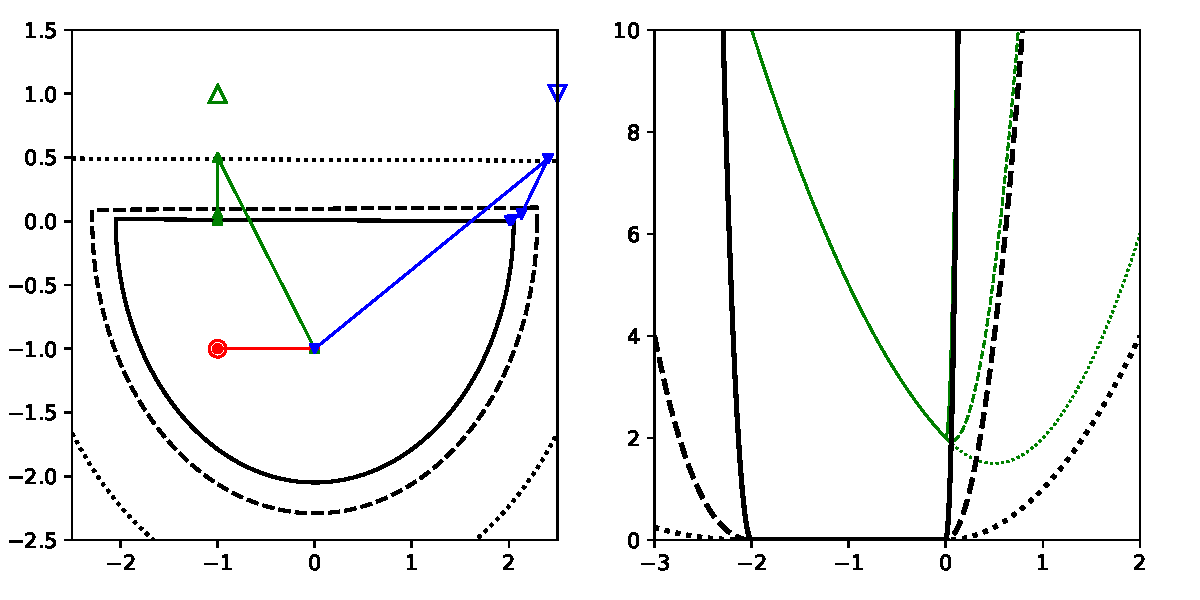
\includegraphics[width=\textwidth]{plots/penalty}
  \caption{Straffunktionsverfahren für einen Halbkreis. Die
    durchgezogenen, gestrichelten, und gepunkteten Linien markieren
    $p_{\sigma}(x)=\nicefrac{1}{2}$ in den Schritten 1,2 und 5. Minimiert wird
    jeweils der Abstand zum den mit offenen Symbolen markierten drei
    Punkten. Der rote Kreis liegt im inneren, das Verfahren braucht
    nur einen Aufruf des freien Optimierers. Für die grünen und blauen
    Dreiecke sind jeweils mehrere Aufrufe nötig, wobei das blaue, nach
    unten zeigende Dreieck so gewählt ist, dass das Minimum in der
    Ecke liegt. Im rechten Graphen sind die Straffunktionen entlang
    der $y$-Achse, also $p_{\sigma}(0,y)$, für die selben Schritte
    gezeigt. Dünner grün sind die korrespondieren Zielfunktionen
    $q_{\sigma}(0,y)$ eingezeichnet.}
  \label{fig:penalty}
\end{figure}

Um das Minimum zu finden, starten wir mit recht kleinem
$\sigma_0>0$. Auf $q_{\sigma}$ wenden wir dann ein
Optimierungsverfahren für freie Optimierung an, etwa das Verfahren des
steilsten Abstiegs mit Schrittweitensteuerung. Aufgrund der
Konstruktion ist der Gradient von $q_{\sigma}$ recht einfach zu berechnen:
\begin{equation}
  \nabla q_{\sigma}(x) = \nabla f(x) + \sum_{i=1}^m 2\sigma\min(0,
  \sigma g_i(x))\nabla g_i(x).
\end{equation}

Sinnvollerweise wählt man einen Startpunkt im Inneren von $M$. Ist im
gefundenen, freien Minimum von $q$ bereits $g_i(x)\ge - \tau$ mit
gewünschter Toleranz $\tau$ erfüllt, ist das Minimum gefunden, und
liegt sehr wahrscheinlich im Inneren vom $M$. Ansonsten wird
$\sigma_k$ erhöht und erneut die Minimierung gestartet, allerdings
naheliegenderweise mit dem bereits gefundenen Minimum als
Startwert. Die Lage des Minimums ändert sich dabei, da ja wegen der
Abbruchbedingung wenigstens eine Nebenbedingung noch nicht erfüllt
war, und sich diese durch die Änderung von $\sigma_k$ ändert. Solange
danach $g_i(x)\ge - \tau$ nicht erreicht ist, passen wir $\sigma_k$ an
und iterieren weiter.

$\sigma_k$ kann auf verschiedene Weisen gewählt werden, solange
$\sigma_k\to \infty$ für $k\to\infty$. Eine Möglichkeit ist etwa
$\sigma_k=k^a$ , wobei man $a>1$ nicht zu groß wählen sollte, zum
Beispiel $a=2$.

Abbildung~\ref{fig:penalty} illustriert das Verfahren am Beispiel
einer Abstandsminimierung zu einem Halbkreis. Wir suchen also
\begin{equation}
  \min_{x\in M} \norm{x - p}_2\quad\text{mit}\;
  M = \{ x | g_i(x) \ge 0, i=1,2 \}
\end{equation}
mit
\begin{equation*}
  g_1(x) = 4 - x^Tx\quad\text{und}\; g_2(x) = -10y.
\end{equation*}
Dies entspricht offenbar $\norm{x}^2_2\le 4$ und $y<0$, also dem
Halbkreis. Im Beispiel werden drei verschiedene Punkte betrachtet und
mit Hilfe des Straffunktionsverfahrens und einem
schrittweitengesteuerten Gradientenverfahren der minimale Abstand zum
Halbkreis gesucht. Der Straffaktor $\sigma$ wurde als $0,1\,k^2$
gewählt, mit $k=1,2,\ldots$ der Iterationsnummer. Für $p=(-1,\,-1)$
liegt das Minimum im Inneren des Halbkreises und wird daher gleich im
ersten Optimierungsschritt gefunden. Für die beiden anderen Punkte,
$p=(-1,\,1)$ und $p=(2,5,\,1)$, sind nur die Gerade beziehungsweise beide
Ungleichungen gleichzeitig aktiv; auch diese Minima werden
gefunden. Auf der rechten Seite sieht man, dass die Straffunktionen
sehr steil werden. Daher ist eine Schrittweitensteuerung hier
besonders wichtig.

\section{Lineare Programme und Simplexalgorithmus}
\index{lineares Programm}
\index{Simplexalgorithmus}

Wie wir in der Einleitung gesehen hatten, führt die lineare Regression
mit Maximumsnorm zu einem ganz anderen Typ von Problemen, bei dem die
Zielfunktion linear ist. Dadurch liegt das Minimum notwendigerweise
auf dem Rand der zulässigen Menge. Sind zusätzlich noch die
Nebenbedingungs(un-)gleichungen linear
(vgl. Abbildung~\ref{fig:simplex}), spricht man von einem
\emph{linearen Programm}. Programm hat hier also erst einmal nichts
mit Computern zu tun. Solche linearen Programme spielen insbesondere
in der Optimierung von Wirtschaftsprozessen eine wichtige Rolle
("`Operations research"'), da Gewinn und produzierte Mengen bei
unverändertem Preis linear von einander abhängen.

\begin{figure}
  \centering
  \begin{tikzpicture}[x=8em,y=8em]
    \draw[->] (-0.1,0) -- (1.2,0);
    \draw[->] (0,-0.1) -- (0,1.2);

    % zulässiger Bereich
    \draw (1,0) -- (0,1) ;
    \fill[pattern=north east lines,rotate around={135:(1,0)}] (1,0) rectangle +(1.414,-0.1) ;
    \fill[pattern=north east lines] (0,0) rectangle +(1,-0.1) ;
    \fill[pattern=north east lines] (0,0) rectangle +(-0.1,1) ;

    % Zielfunktion
    \pgfmathsetmacro{\gradx}{0.3}
    \pgfmathsetmacro{\grady}{-0.4}
    \pgfmathsetmacro{\perpx}{\grady}
    \pgfmathsetmacro{\perpy}{-\gradx}

    \draw[very thick,->=triangle 45] (0.2,0.6) -- +(\gradx,\grady);

    % Isolinien
    \foreach \l in {0,0.2,0.4,...,0.8} {
      \pgfmathsetmacro{\ll}{(1-\l)/(\perpx+\perpy)}     
      \draw (0, \l) -- (\ll*\perpx,\l+\ll*\perpy);
    }

    \foreach \l in {0.2,0.2,0.4,...,0.8} {
      \pgfmathsetmacro{\ll}{(1-\l)/(\perpx+\perpy)}     
      \draw (\l, 0) -- (\l + \ll*\perpx, \ll*\perpy);
    }

    % Minimum
    \filldraw (1, 0) circle (0.04);

  \end{tikzpicture}
  \hspace{4em}
  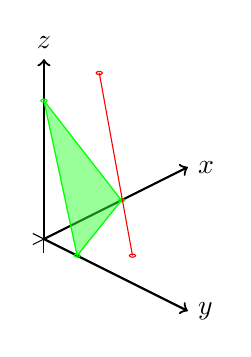
\begin{tikzpicture}[x={(4em,2em)},y={(4em,-2em)},z={(0em,5em)}]
    \draw (xyz cs:x=-.1) -- (xyz cs:x=0);
    \draw (xyz cs:y=-.1) -- (xyz cs:y=0);
    \draw (xyz cs:z=-.1) -- (xyz cs:z=0);

    \draw[thick,->] (xyz cs:x=0) -- (xyz cs:x=1.3) node[right] {$x$};
    \draw[thick,->] (xyz cs:y=0) -- (xyz cs:y=1.3) node[right] {$y$};
    \draw[thick,->] (xyz cs:z=0) -- (xyz cs:z=1.3) node[above] {$z$};

    \draw[color=green,fill=green!80!white,opacity=0.5]
    (xyz cs:z=1) -- (xyz cs:x=0.7) -- (xyz cs:y=0.3) -- cycle;
    \draw[color=green]
    (xyz cs:z=1) -- (xyz cs:x=0.7) -- (xyz cs:y=0.3) -- cycle;

    \draw[color=green]
    (xyz cs:z=1) circle (0.02)
    (xyz cs:x=0.7) circle (0.02)
    (xyz cs:y=0.3) circle (0.02);

    \draw[color=red]
    (xyz cs:z=1,x=0.5) -- (xyz cs:z=0.2,y=0.8);

    \draw[color=red]
    (xyz cs:z=1,x=0.5)   circle (0.02)
    (xyz cs:z=0.2,y=0.8) circle (0.02);
  \end{tikzpicture}
  \caption{Links: Illustration eines linearen Programms. Die
    Nebenbedingungen sind $x\ge 0$, $y\ge 0$ und $1 - x \ge y$. Der
    Pfeil deutet die Abstiegsrichtung an, die Linien sind Isolinien
    des Potentials. Hier findet sich das Minimum in der mit einem
    Punkt markierten rechten unteren Ecke. Rechts: 3d-Simplex mit
    Nebenbedingung. Ist eine Nebenbedingung $a^Tx=b$ gegeben, so sind
    nur Punkte mit Koordinaten $\ge 0$ aus dieser Ebene zulässig, also
    aus dem grünen Dreieck. Die Ecken lassen sich durch die Menge der
    Koordinaten, die nicht Null sind, vollständig beschreiben. Die
    unterste Ecke etwa hat nur $y$ aktiv, die obere $z$. Sind zwei
    Nebenbedingungen gegeben, so ist die resultierende zulässige Menge
    eine Gerade (hier rot eingezeichnet). Die Ecken werden nun durch
    zwei aktive Koordinaten beschrieben, hier $y$ und $z$ für die
    vordere Ecke, und $x$ und $z$ für die hintere.}
  \label{fig:simplex}
\end{figure}

Lineare Programme können in einer Vielzahl von Formen definiert
werden, wir betrachten hier die Normalform
\begin{equation}
  \label{eq:simplexprob}
  \min c^Tx \quad\text{unter den Nebenbedingungen}\; x\ge 0,\;Ax=b
\end{equation}
mit $c\in\RR^n$, $A\in\RR^{m,n}$ und $b\in\RR^{m}$. Die Anzahl $m$ der
Gleichungsbedingungen ist dabei nicht festgelegt. Da $x$ ein Vektor
ist, bedeutet $x\ge 0$ einfach, dass alle Komponenten größer als Null
sein sollen. Alle linearen Nebenbedingungen lassen sich so
formulieren, eventuell unter Zuhilfenahme von weiteren Variablen.

Betrachten wir zwei Beispiele. Die in der Abbildung~\ref{fig:simplex}
gegebene Nebenbedingung $1 - x \ge y$ ist offensichtlich nicht von der
obigen Form. Wir führen deswegen eine neue Variable $z=1-x-y$ ein, die
offenbar $z\ge 0$ erfüllen muss. Wir erhalten dann die Normalform mit
$c'=(c_0, c_1, 0)$, da $z$ ja nicht zur eigentlich Zielfunktion
beiträgt, sowie $A=(-1,-,1, -1)$ und $b=-1$.

Auch \eqref{eq:chebyshevappr} für die lineare Regression mit
Maximumsnorm ist nicht in Normalform. Zum einen müssen wir die
Nebenbedingungsungleichungen in Gleichungen transformieren. Dazu
führen wir einfach eine Schattenvariable $z_i=a_i^Tv - b_i$ pro
Ungleichung $a_i^Tv\ge b_i$ ein. Dann ist $z_i\ge 0$ offenbar
äquivalent zur Ungleichung. Zum anderen sind aber die Variablen $v$
frei, während wir voraussetzen, dass $v\ge 0$. Um dies zu beheben,
teilen wir jede Variable $v=v_+ - v_i$ auf und ergänzen $A$ und $c$
entsprechend. Dadurch transformiert sich
\begin{equation}
  \min_v (0,\ldots,\,0,\,1)^T v\quad\text{unter der Bedingung}\;
  \begin{pmatrix}
    A & e\\
    -A & e
  \end{pmatrix} v \ge
  \begin{pmatrix}
    b\\
    -b
  \end{pmatrix}
\end{equation}
in die äquivalente Aufgabe
\begin{equation}
  \min_x (\tikzlabel{vpl}0,\ldots,\,0,\,1\tikzlabel{vpr},
  \tikzlabel{vml}0,\ldots,\,0,\,-1\tikzlabel{vmr},
  \tikzlabel{zl}0,\ldots,\,0\tikzlabel{zr})^T v
\end{equation}
\begin{tikzpicture}[overlay, remember picture]
  \draw[decorate,decoration=brace] ($(vpl) + (0,1em)$) --
  node[above] {$v_+$} ($(vpr) + (0,1em)$);
  \draw[decorate,decoration=brace] ($(vml) + (0,1em)$) --
  node[above] {$v_-$} ($(vmr) + (0,1em)$);
  \draw[decorate,decoration=brace] ($(zl) + (0,1em)$) --
  node[above] {$z$} ($(zr) + (0,1em)$);
\end{tikzpicture}
mit der neuen Variablen $x=(v_+,v_-,z)$ und den Nebenbedingungen $x\ge 0$
und
\vspace{0.5em}% für die TikZ-Deko
\begin{equation*}
  \begin{pmatrix}
    \tikzlabel{vpl}A  & e\tikzlabel{vpr} & 
    \tikzlabel{vml}-A & -e\tikzlabel{vmr} &
    \tikzlabel{zl} I & 0\tikzlabel{zr}\\
    -A & e &  A & -e & 0 & I
  \end{pmatrix}
  x =
  \begin{pmatrix}
    b\\
    -b
  \end{pmatrix}.
\end{equation*}
\begin{tikzpicture}[overlay, remember picture]
  \draw[decorate,decoration=brace] ($(vpl) + (0,1em)$) --
  node[above] {$v_+$} ($(vpr) + (0,1em)$);
  \draw[decorate,decoration=brace] ($(vml) + (0,1em)$) --
  node[above] {$v_-$} ($(vmr) + (0,1em)$);
  \draw[decorate,decoration=brace] ($(zl) + (0,1em)$) --
  node[above] {$z$} ($(zr) + (0,1em)$);
\end{tikzpicture}

Wie können wir Aufgabe \eqref{eq:simplexprob} lösen? Sofern die
zulässige Menge beschränkt ist, beschreiben die Nebenbedingungen immer
einen Polyeder. Man kann nun zeigen, dass sich ein Optimum immer in
einer der Ecken dieses Polyeders befindet. Der Simplex-Algorithmus
besucht nun nacheinander die Ecken des Polyeders, so dass die
Zielfunktion fortlaufend minimiert wird. Daher zerfällt der
Algorithmus in zwei Phasen. In der ersten Phase muss eine gültige Ecke
bestimmt werden, in der zweiten Phase müssen wir dann von einer
gültigen Ecke aus eine neue, benachbarte Ecke mit niedrigerer
Zielfunktion finden.

\subsubsection*{Phase II}

Wir beginnen mit der zweiten Phase, da die die erste Phase letztlich
auf denselben Ideen beruht. Wir nehmen daher an, dass die Matrix $A$
maximalen Zeilenrang hat, also alle doppelten Gleichung eliminiert
wurden; dies wird später die erste Phase automatisiert übernehmen.
Außerdem sei $x$ eine Ecke des Polyeders.

Wie stellen wir diese Ecke dar? Abbildung~\ref{fig:simplex}
illustriert, dass die Ecken einfach durch die Menge der aktiven, also
von Null verschiedenen Koordinaten beschrieben werden kann. Da wir
angenommen haben,dass $A\in\RR^{m,n}$ linear unabhängige Zeilen hat,
beschreibt $Ax=b$ einen $n-m$-dimensionalen Unterraum, dessen Ecken
durch jeweils $m$ aktive Koordinaten haben. Sei $B=\{j_1,\ldots,k_m\}$
die Menge der aktiven Koordinaten, die sogenannten Basiskoordinaten,
und $N=\{1,\ldots,n\}\backslash B$ die Menge der
Nichtbasiskoordinaten. $A_B = (a_{j_1},\ldots,a_{j_m})\in\RR^{m,m}$
sei die zu den Basisvariablen $x_B = (x_{j_i})_i\in\RR^m$ gehörende
Teilmatrix, sowie $A_N$ analog die zu den Nichtbasisvariablen
gehörende Teilmatrix. Dann gilt $x_N=0$ und damit $A_Bx_b = b$.

Damit ist der Zielfunktionswert in $x$
*\begin{equation}
  c^Tx = c_B^Tx_B = c_BA_B^{-1}b
\end{equation}
Wir betrachten nun eine beliebigen anderen Punkt $u\in M$, also $u\ge
0$ und $Au=A_Bu_B + A_Nu_N = b$. Dann ist
\begin{equation}
  \label{eq:simplexub}
  u_b = A_B^{-1}(b-A_Nu_N) = x_B - A_B^{-1}A_Nu_N
\end{equation}
und damit
\begin{equation}
  c^Tu = c_B^T(x_B - A_B^{-1}A_Nu_N) + c_N^Tu_N = c^Tx +
  \underbrace{(c_N - A_B^{-1}A_Nu_N)^T}_{r}u_n.
\end{equation}
Da $u_N\ge 0$ ist, kann die Zielfunktion nur verkleinert werden, wenn
eine Komponente $r_s < 0$ ist. Ist dies nicht der Fall, haben wir also
unser Optimum gefunden.

Sei nun also $r_s< 0$. Dann können wir unser Ergebnis verbessern, in
dem wir $u_s>0$ wählen, aber alle anderen Elemente von $u_N$ weiterhin
bei 0 belassen. Wir nehmen also $s$ in die Basiskoordinaten $B$
auf. Damit diese eine Basis bleiben, müssen wir nun noch sehen, welche
Gleichung dafür herausfällt. Aus \eqref{eq:simplexub} folgt, dass dann
$u_B = x_B - u_s A_B^{-1}a_s$ und
\begin{equation}
  \label{eq:simplextgt}
  c^Tu = c^Tx + u_s(c_s - c_B^T A_B^{-1}a_s)
\end{equation}
Auch im neuen Punkt muss aber $u_B\ge
0$ gelten, daher können wir $u_N$ nur so groß wählen, bis für die erste
Basisvariable $x_t= u_s (A_B^{-1}a_s)_t$ gilt. Dann gilt $u_t=0$,
d.h. diese Basisvariable geht in die Nichtbasis über.

Wir suchen also
\begin{equation}
  u_s = \min \left\{\frac{x_{j_k}}{(A_B^{-1}a_s)_k} | k\in B,
      (A_B^{-1}a_s)_k > 0\right\} =:
  \frac{x_{j_t}}{(A_B^{-1}a_s)_t}
\end{equation}
Sind dabei alle $(A_B^{-1}a_s)_k < 0$, so dass das Minimum gar nicht
existiert, können wir $u_B$ unbegrenzt groß machen, also ist der
zulässige Bereich unbeschränkt, und wir müssen abbrechen, da die
Funktion beliebig klein werden kann.

Wir tauschen nun in der Basis $B$ $j_t$ durch $s$ aus und erhalten die
neue Basis $B'$. Für die Rechnungen benötigen wir nur $A_B^{-1}$, dass
wir nun entsprechend anpassen müssen. Dies können wir mit Hilfe der
Sherman-Morrison-Formel sehr bequem ähnlich einem Schritt der
Gaußelimination berechnen:
\begin{equation}
  \label{eq:simplexex}
  A_{B'}^{-1} = A_{B}^{-1} - \frac{A_B^{-1}a_s - e_t}{(A_B^{-1}a_s)_t}
  \left(e_t^TA_{B}^{-1}\right)
\end{equation}

\subsubsection*{Phase I}

Wie können wir nun eine zulässige erste Lösung mit zugehörigem
Basissatz und $A_B^{-1}$ finden? Die Idee ist, zunächst die Matrix
noch einmal stark zu erweitern, sodass eine gültige Lösung einfach zu
finden ist, aber jede echte gültige Lösung günstiger. Daher fallen die
zusätzlichen Variablen alle in die Nichtbasis und können eliminiert
werden.

Dazu betrachten wir also das neue Problem
\begin{equation}
  \min_z (\tikzlabel{xl}0,\ldots,\,0,\tikzlabel{xr},
  \tikzlabel{yl}1,\ldots,\,1\tikzlabel{yr})^Tz
\end{equation}
\begin{tikzpicture}[overlay, remember picture]
  \draw[decorate,decoration=brace] ($(xl) + (0,1em)$) --
  node[above] {$x$} ($(xr) + (0,1em)$);
  \draw[decorate,decoration=brace] ($(yl) + (0,1em)$) --
  node[above] {$y$} ($(yr) + (0,1em)$);
\end{tikzpicture}
mit der neuen Variablen $z=(x,y)$ und den Nebenbedingungen $z\ge 0$
und
\begin{equation*}
  \begin{pmatrix}
    \tilde{A} & I 
  \end{pmatrix}
  z =
  \begin{pmatrix}
    \tilde{b}
  \end{pmatrix}.
\end{equation*}
Dabei sind die $i$-ten Zeilen von $\tilde{A}$ und $\tilde{b}$
identisch mit denen von $A$ und $b$, nur werden die Vorzeichen
getauscht, falls $b_i<0$. Da also nur einige Zeilen mit $-1$
multipliziert werden, wird die Lösung des Gleichungssystems nicht
verändert, aber es gilt $\tilde{b}\ge 0$.

Sofern die ursprüngliche zulässige Menge nicht leer war, ist das
Minimum dieser Zielfunktion offenbar Null, nämlich dann, wenn alle
$y=0$ sind. Andererseits kennen wir einen zulässigen Punkt des neuen
Problems, nämlich $(0,\tilde{b})$. Außerdem hat die Matrix zu $z$
maximalen Zeilenrang aufgrund der zu $y$ gehörigen Identität. Wir
können also die Phase I des Simplex-Algorithmus unmittelbar auf diese
Matrix anwenden.

Findet der Simplex-Algorithmus nun ein Minimum, dass von Null
verschieden ist, ist offenbar die ursprüngliche zulässige Menge leer
gewesen, und wir müssen abbrechen. Ist das Minimum hingegen Null und
alle $y=0$, also in der Nichtbasis, so haben wir unseren Startwert für
die Phase II gefunden. Es kann allerdings auch passieren, dass noch zu
$y$ gehörige Indizes $j_t>n$ in der Basis vorkommen. Dann müssen wir
eine echte Koordinate $s<n$ finden, die mit $j_t$ getauscht werden
kann. Dazu müssen wir ein $s$ mit $A_B^{-1}a_s)_t\neq 0$ finden, so
dass wir wieder unsere Austauschformel \eqref{eq:simplexex} anwenden
können. Finden wir diese nicht, dann kann man zeigen,dass die
ursprüngliche Matrix nicht linear unabhängig gewesen war. In diesem
Fall wird die $j_t-n$-te Zeile gestrichen.

%\section{Globale Optimierung}
%\subsection{Simulated annealing}
%\subsection{Genetische Algorithmen}

%%% Local Variables: 
%%% mode: latex
%%% TeX-master: "padc.tex"
%%% TeX-PDF-mode: t
%%% End: 
